%
% teil2.tex -- Hankel-Kontur
%
% (c) 2026 Jannis Gull, OST Ostschweizer Fachhochschule
%
% !TEX root = ../../buch.tex
% !TEX encoding = UTF-8
%

\section{Die Hankel-Kontur
\label{hankel:section:hankel}}
\kopfrechts{Die Hankel-Kontur}

Die Mellin-Darstellung scheitert nur an der Singularität im Ursprung. 
\index{Hankel-Kontur}%
Die Grundidee der Hankel-Kontur besteht darin, diesen Punkt in der komplexen Ebene zu umgehen. 
Dabei entsteht allerdings eine neue Frage: Der Integrand enthält eine komplexe Potenz.
Eine solche Potenz ist erst festgelegt, nachdem ein Zweig des komplexen Logarithmus gewählt worden ist.

\subsection{Hauptzweig und Verzweigungsschnitt}

Für $w\in\mathbb C\setminus(-\infty,0]$ wird der Hauptzweig des Logarithmus durch
\begin{equation}
\log w
=
\log|w|+i\operatorname{arg}(w),
\qquad
-\pi<\operatorname{arg}(w)<\pi
\label{hankel:eq:hauptzweig-log}
\end{equation}
definiert. 
Die komplexe Potenz im späteren Konturintegral wird damit als
\begin{equation}
(-z)^{s-1}
=
\exp((s-1)\log(-z))
\label{hankel:eq:minus-z-potenz}
\end{equation}
beschrieben. 
Weil der Logarithmus auf $-z$ angewendet wird, wird der
Verzweigungsschnitt in der $z$-Ebene von der negativen auf die positive reelle Achse gespiegelt.

Für einen Punkt $x>0$ besitzt $-z$ oberhalb und unterhalb dieses Schnittes unterschiedliche Argumente. 
Nähert man sich der positiven Achse von oben, $z=x+i0$, so liegt $-z$ knapp unterhalb der negativen Achse und hat das
Argument $-\pi$. 
Daher ist
\begin{equation}
\log(-(x+i0))
=
\log x-i\pi.
\label{hankel:eq:log-oben}
\end{equation}
Nähert man sich dagegen von unten, $z=x-i0$, so liegt $-z$ knapp oberhalb der negativen Achse und hat das Argument $+\pi$:
\begin{equation}
\log(-(x-i0))
=
\log x+i\pi.
\label{hankel:eq:log-unten}
\end{equation}
Für die komplexen Potenzen ergeben sich damit die beiden Randwerte
\begin{equation}
(-(x+i0))^{s-1}
=
x^{s-1}e^{-i\pi(s-1)}
\label{hankel:eq:potenz-oben}
\end{equation}
und
\begin{equation}
(-(x-i0))^{s-1}
=
x^{s-1}e^{i\pi(s-1)},
\label{hankel:eq:potenz-unten}
\end{equation}
dargestellt in Abbildung~\ref{hankel:fig:phasensprung}.
Die beiden Werte unterscheiden sich nur durch ihre Phasen. Diese Phasendifferenz erzeugt später den Sinusfaktor. 
Ohne den Verzweigungsschnitt würden sich die Beiträge der beiden geraden Konturstücke wegen ihrer entgegengesetzten Orientierung aufheben.

\input{papers/hankel/fig/fig-phasensprung.tex}
%\begin{figure}
%	\centering
%	\begin{tikzpicture}[scale=1.2,>=latex]
%		% Achsen
%		\draw[->] (-0.8,0) -- (5.4,0) node[right] {$\Re(z)$};
%		\draw[->] (0,-1.4) -- (0,1.8) node[above] {$\Im(z)$};
%		\draw[very thick,red] (0,0) -- (5.0,0);
%		% Parameter
%		\def\eps{0.6}
%		
%		% oberer und unterer Teil der Hankel-Kontur
%		\draw[->,thick] (\eps,0.12) -- (4.8,0.12);
%		\draw[->,thick] (4.8,-0.12) -- (\eps,-0.12);
%		
%		\node[above] at (3.2,0.18) {$x^{s-1}e^{-i\pi(s-1)}$};
%		\node[below] at (3.2,-0.18) {$x^{s-1}e^{+i\pi(s-1)}$};
%	\end{tikzpicture}
%	\caption{Die unterschiedlichen Randwerte von $(-z)^{s-1}$ oberhalb und
%		unterhalb des rot markierten positiven Verzweigungsschnittes.}
%	\label{hankel:fig:phasensprung}
%\end{figure}

\subsection{Verlauf und Orientierung der Kontur}

Die Hankel-Kontur $H$ läuft von $+\infty$ knapp unterhalb der positiven reellen Achse zum Ursprung, umrundet den Ursprung im Uhrzeigersinn auf einem kleinen Kreis $C_\varepsilon$ und kehrt knapp oberhalb der positiven Achse nach $+\infty$ zurück. 
Dies ist Abbildung in~\ref{hankel:fig:hankelkontur} dargestellt. 
Es ist wichtig, die Orientierung beider Äste zu beachten: Auf dem unteren Ast nimmt $x$ ab, auf dem oberen Ast nimmt $x$ zu.

%
% fig-hankelkontur.tex
%
% (c) 2026 Prof Dr Andreas Müller
%
\begin{figure}
\centering
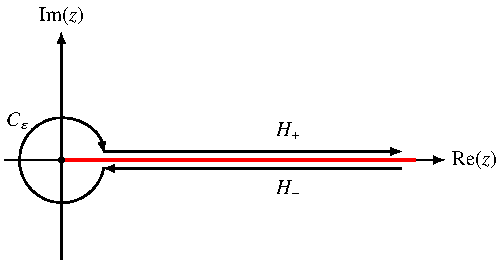
\includegraphics{papers/hankel/images/hankelkontur.pdf}
%\begin{tikzpicture}[scale=1.2,>=latex]
%	% Achsen
%	\draw[->] (-0.8,0) -- (5.4,0) node[right] {$\Re(z)$};
%	\draw[->] (0,-1.4) -- (0,1.8) node[above] {$\Im(z)$};
%	\draw[very thick,red] (0,0) -- (5.0,0);
%	% Parameter
%	\def\eps{0.6}
%	
%	% oberer und unterer Teil der Hankel-Kontur
%	\draw[->,thick] (\eps,0.12) -- (4.8,0.12);
%	\draw[->,thick] (4.8,-0.12) -- (\eps,-0.12);
%	
%	% kleiner Kreis um 0
%	\draw[<-,thick] (\eps,0.1) arc[start angle=10,end angle=350,radius=\eps];
%	
%	% Ursprung
%	\fill (0,0) circle[radius=1.2pt];
%	
%	\node[above] at (3.2,0.18) {$H_+$};
%	\node[below] at (3.2,-0.18) {$H_-$};
%	\node[left] at (-0.35,0.55) {$C_\varepsilon$};
%\end{tikzpicture}
\caption{Die Hankel-Kontur um den positiven Verzweigungsschnitt.}
\label{hankel:fig:hankelkontur}
\end{figure}

%\begin{figure}
%\centering
%\begin{tikzpicture}[scale=1.2,>=latex]
%	% Achsen
%	\draw[->] (-0.8,0) -- (5.4,0) node[right] {$\Re(z)$};
%	\draw[->] (0,-1.4) -- (0,1.8) node[above] {$\Im(z)$};
%	\draw[very thick,red] (0,0) -- (5.0,0);
%	% Parameter
%	\def\eps{0.6}
%	
%	% oberer und unterer Teil der Hankel-Kontur
%	\draw[->,thick] (\eps,0.12) -- (4.8,0.12);
%	\draw[->,thick] (4.8,-0.12) -- (\eps,-0.12);
%	
%	% kleiner Kreis um 0
%	\draw[<-,thick] (\eps,0.1) arc[start angle=10,end angle=350,radius=\eps];
%	
%	% Ursprung
%	\fill (0,0) circle[radius=1.2pt];
%	
%	\node[above] at (3.2,0.18) {$H_+$};
%	\node[below] at (3.2,-0.18) {$H_-$};
%	\node[left] at (-0.35,0.55) {$C_\varepsilon$};
%\end{tikzpicture}
%\caption{Die Hankel-Kontur um den positiven Verzweigungsschnitt.}
%\label{hankel:fig:hankelkontur}
%\end{figure}

Betrachtet wird das Integral
\begin{equation}
I(s)
=
\int_H
\frac{(-z)^{s-1}}{e^z-1}
\,dz.
\label{hankel:eq:hankel-integral}
\end{equation}
Vorerst wird die Beziehung zur Mellin-Darstellung weiterhin unter der Voraussetzung $\operatorname{Re}(s)>1$ hergeleitet. In diesem Gebiet darf der Radius $\varepsilon$ gegen null geführt werden.

\subsection{Der Beitrag des kleinen Kreises}

Auf dem Kreis $|z|=\varepsilon$ wird die Exponentialfunktion am Ursprung entwickelt:
\begin{equation}
e^z-1
=
z+O(z^2)
=
z(1+O(z)).
\label{hankel:eq:exp-klein}
\end{equation}
Der Nenner verhält sich dort also wie $z$. 
Für $s=\sigma+it$ hat der Zähler die Grössenordnung $|z|^{\sigma-1}$; der zusätzliche Faktor, der aus dem
Argument von $-z$ entsteht, ist auf dem festen Kreis für ein festes $s$ beschränkt. 
Damit existiert eine Konstante $C_s>0$ mit
\begin{equation}
\biggl|
\frac{(-z)^{s-1}}{e^z-1}
\biggr|
\leq
C_s\varepsilon^{\operatorname{Re}(s)-2}.
\label{hankel:eq:kleiner-kreis-majorante}
\end{equation}
Da der Kreis $C_\rho$ die Länge $2\pi\rho$ besitzt, ist der Betrag des Integrals höchstens das Produkt aus dieser Länge und dem maximalen Betrag des Integranden auf dem Kreis. 
Aus \eqref{hankel:eq:kleiner-kreis-majorante} folgt somit
\begin{equation}
\biggl|
\int_{C_\varepsilon}
\frac{(-z)^{s-1}}{e^z-1}
\,dz
\biggr|
\leq
2\pi C_s\varepsilon^{\operatorname{Re}(s)-1}.
\label{hankel:eq:kleiner-kreis-ml}
\end{equation}
Für $\operatorname{Re}(s)>1$ ist der Exponent positiv und der rechte Ausdruck geht für $\varepsilon\to0$ gegen null. 
An dieser Stelle tritt somit dieselbe Bedingung auf wie bei der Mellin-Darstellung. 
Für die Herleitung der Hankel-Formel ist das zunächst ausreichend.

\subsection{Die beiden geraden Äste}

Auf dem unteren Ast wird $z=x-i0$ parametrisiert. 
Die Orientierung verläuft von einem grossen $R$ nach $\varepsilon$. 
Mit \eqref{hankel:eq:potenz-unten} ergibt sich
\begin{equation}
\begin{aligned}
\int_{H_-}
\frac{(-z)^{s-1}}{e^z-1}\,dz
&=
e^{i\pi(s-1)}
\int_R^\varepsilon
\frac{x^{s-1}}{e^x-1}\,dx
\\
&=
-
e^{i\pi(s-1)}
\int_\varepsilon^R
\frac{x^{s-1}}{e^x-1}\,dx.
\end{aligned}
\label{hankel:eq:unterer-ast}
\end{equation}
Auf dem oberen Ast gilt $z=x+i0$ und die Orientierung läuft von
$\varepsilon$ nach $R$. 
Daher
\begin{equation}
\int_{H_+}
\frac{(-z)^{s-1}}{e^z-1}\,dz
=
e^{-i\pi(s-1)}
\int_\varepsilon^R
\frac{x^{s-1}}{e^x-1}\,dx.
\label{hankel:eq:oberer-ast}
\end{equation}
Nach Addition der beiden Beiträge bleibt derselbe reelle Integralterm übrig,
während die Phasen voneinander subtrahiert werden:
\begin{equation}
\begin{aligned}
&\int_{H_-}
\frac{(-z)^{s-1}}{e^z-1}\,dz
+
\int_{H_+}
\frac{(-z)^{s-1}}{e^z-1}\,dz
\\
&\qquad=
\Bigl(
e^{-i\pi(s-1)}-e^{i\pi(s-1)}
\Bigr)
\int_\varepsilon^R
\frac{x^{s-1}}{e^x-1}\,dx.
\end{aligned}
\label{hankel:eq:beide-aeste}
\end{equation}
Mit der Identität $e^{-i\alpha}-e^{i\alpha}=-2i\sin\alpha$ und
$\sin(\pi(s-1))=-\sin(\pi s)$ folgt
\begin{equation}
e^{-i\pi(s-1)}-e^{i\pi(s-1)}
=
2i\sin(\pi s).
\label{hankel:eq:phasen-differenz}
\end{equation}
Nun werden zuerst $R\to\infty$ und anschliessend $\varepsilon\to0$ geführt.
Der kleine Kreis verschwindet für $\operatorname{Re}(s)>1$, und das reelle Integral wird nach \eqref{hankel:eq:mellin-darstellung} zu $\Gamma(s)\zeta(s)$. Damit ist
\begin{equation}
I(s)
=
2i\sin(\pi s)\Gamma(s)\zeta(s).
\label{hankel:eq:hankel-mellin}
\end{equation}

\subsection{Die Hankel-Darstellung der Zetafunktion}

Die Reflexionsformel der Gamma-Funktion
\begin{equation}
\Gamma(s)\Gamma(1-s)
=
\frac{\pi}{\sin(\pi s)}
\label{hankel:eq:reflexionsformel}
\end{equation}
ist in~\cite{hankel:dlmf} genau in der Form angegeben, welche hier benötigt wird. 
Aus ihr folgt
\begin{equation}
\sin(\pi s)\Gamma(s)
=
\frac{\pi}{\Gamma(1-s)}.
\label{hankel:eq:reflexion-umgestellt}
\end{equation}
Einsetzen in \eqref{hankel:eq:hankel-mellin} ergibt
\begin{equation}
I(s)
=
\frac{2\pi i}{\Gamma(1-s)}\zeta(s),
\label{hankel:eq:hankel-vor-endformel}
\end{equation}
und damit schliesslich
\begin{equation}
\boxed{
\zeta(s)
=
\frac{\Gamma(1-s)}{2\pi i}
\int_H
\frac{(-z)^{s-1}}{e^z-1}
\,dz.
}
\label{hankel:eq:hankel-darstellung}
\end{equation}
Diese Hankel-Darstellung findet sich in äquivalenter Form
beispielsweise in \cite{hankel:dlmf}.

Bis zu diesem Punkt wurde die Formel aus der Mellin-Darstellung für $\operatorname{Re}(s)>1$ abgeleitet. 
Der wesentliche Gewinn liegt aber darin, dass das Konturintegral anders behandelt werden kann als das ursprüngliche reelle Integral. 
Für die Herleitung wurde der kleine Kreis gegen null
geführt, für die analytische Fortsetzung wird sein Radius stattdessen fest gehalten. 
Dadurch bleibt die Kontur vom problematischen Punkt $z=0$
getrennt. 
Für $0<\varepsilon<2\pi$ kann der Radius des kleinen Kreises verändert werden, ohne dass eine Singularität des Integranden überquert wird. 
Zwei solche Hankel-Konturen lassen sich im geschlitzten Gebiet stetig ineinander deformieren. 
Nach dem cauchyschen Integralsatz ist das Konturintegral daher unabhängig vom gewählten Radius $\varepsilon$. 
\index{Satz!Cauchy-Integralsatz}%
Für die Fortsetzung darf $\varepsilon$ somit fest positiv gewählt werden.
Genau dieser Wechsel ist der Inhalt des nächsten Abschnitts.
